\documentclass[12pt]{article}
\usepackage{lineno}
\linenumbers
\usepackage{setspace}
\doublespacing
\usepackage[english]{babel}
\usepackage[utf8x]{inputenc}
\usepackage{amsmath}
\usepackage{graphicx}
\usepackage{authblk}
\usepackage{natbib}
\usepackage{hyperref}
\usepackage[margin=1in]{geometry}
\bibpunct{(}{)}{;}{author-year}{}{,}

\title{Host diversity begets symbiont diversity and reduces transmission}

\author[1]{Maxwell B. Joseph} 
\author[2]{Joseph R. Mihaljevic}
\author[1]{Pieter T. J. Johnson}
\affil[1]{Ecology and Evolutionary Biology, University of Colorado, Boulder, CO}
\affil[2]{Ecology and Evolution, University of Chicago, IL}
\date{}
\renewcommand\Affilfont{\itshape\small}

\begin{document}
\maketitle

\begin{abstract}
Explaining patterns of biodiversity is one of the primary aims of ecology, and historically these patterns have been described in terms of macroorganisms such as plants and animals. 
Recent methodological advances grant the ability to observe previously unobservable microbial communities, which are incredibly diverse and often nested within free-living organisms, providing an impetus and means to expand understanding of the mechanisms that structure communities. 
These mechanisms are potentially similar to the mechanisms that structure free-living communities, with habitat patches for free-living species being analogous to host individuals for symbiotic organisms, often microbial, that live in or on free-living species.
Here, we apply this analogy to explore the possible effects of host functional diversity on symbiotic organisms with a stochastic multi-species model across a range of scenarios including specialist, generalist, parasitic, commensal, and mutualistic symbionts. 
The model predicts that host functional diversity nearly always increases symbiont diversity, though the shape of the increase varies as a function of symbiont niche breadth and the fitness consequences of infection. 
In addition, diverse host communities are predicted to have lower transmission rates on average, and relatively greater transmission of generalist symbionts. 
The same mechanisms allow host diversity to increase symbiont diversity while reducing transmission.
Namely, diverse host communities have higher symbiont colonization rates but fewer hosts available for local transmission, which increases the probability of stochastic symbiont extirpation.
These results are potentially useful as a step toward a more unified community ecology of free-living and symbiotic organisms.
\end{abstract}

\section*{Introduction}
%I like this intro paragraph, but I think it actually limits the scope by referencing microbial data sets. I think we could use this as an example, but really talk about regional patterns of symbiont community composition more broadly. I'll try...


Recent sequencing technologies have increased our capacity to collect community-wide microbial data. 
This has motivated calls to develop theoretical frameworks that explain microbial diversity, borrowing theory developed for free-living species \citep{Prosser2007} %Fierer_etal_2012_AREE, Costello_etal_2012_Science. 
Simultaneously, considerable effort has been invested in developing theory that explicitly links free-living diversity to pathogen transmission dynamics to understand how host diversity affects disease risk \citep{Dobson2004a, Roche2012, Joseph2013a, Mihaljevic2014}. 
Both microbial ecologists and disease ecologists have a shared interest in understanding the relationships between free-living and microbial diversity, but there has been little synthesis between these two camps on this topic. 
Here, we borrow from models of free-living diversity to construct a general model to explore how host diversity affects the transmission and diversity of parasites, mutualists, and commensal symbionts.

Analogies have been drawn between free-living organisms living in habitat patches and symbionts living in host individuals \citep{Mihaljevic2012}. 
In this sense, habitat heterogeneity may be considered analogous to host diversity. 
Habitat heterogeneity is expected to increase colonization opportunities for free-living species, as diverse habitats are more likely to contain resources that can be exploited by any particular species. 
However, for fixed area, as habitat heterogeneity increases, the area of each habitat type must go down because of an inherent trade-off with habitat heterogeneity. 
As a result, mean population sizes have been predicted to decrease with habitat heterogeneity, leading to a higher probabilities of stochastic extinctions. 
The result of these changes in colonization and extinction is predicted to be a unimodal relationship between habitat heterogeneity and free-living species richness. 

Whether these mechanisms could apply to symbionts remains an open question that we investigate here from a theoretical perspective. 
We proceed by developing a computational model for replicate local communities consisting of multiple species of hosts and symbionts. 
Central to this effort is an exploration of how host functional diversity might affect symbiont transmission and richness over a range of cases, including communities with varying symbiont niche breaths - a combination of specialist and generalist symbionts - and varying fitness consequences - a combination of parasites, commensals, and mutualists. 

\section*{Methods}

We developed a stochastic, continuous-time, agent-based model for the dynamics of host-symbiont communities.  In the model, a host community resides in a habitat patch that is divided into a finite number of cells $C$, i.e. micro-sites, in which each cell can be occupied by a single host individual.
Within the habitat patch, host colonization, reproduction, and death occur with rates $c$, $r$, and $d$, respectively, which are constant across model realizations.
Multiple host species $h=1, ..., H$ exist within a regional pool, and the patch experiences a constant rate of host colonization $c$, which is equal for all host species, and there is no displacement of occupying hosts by colonizing hosts. 
Host species vary in traits that are relevant to symbiont infection, but the communities are otherwise neutral, in that all host species have equal colonization, reproduction, and death rates. 
Once a host colonizes a cell, it then has some rate of reproduction and of death that is constant among host species.
Offspring attempt to disperse to a random habitat patch cell, and if it is unnoccupied, they successfully colonize.

Multiple types (species) of symbionts occur in the regional pool and attempt to colonize host individuals with a constant rate $r_s$. 
Host species vary in traits relevant to symbiont establishment probability. 
We assume for simplicity that this variation is unidimensional, as would be the case if there were one primary niche axis for the symbionts, e.g. pH of the host gut.
Symbiont niches are represented as univariate Gaussian functions with niche optima and breadths (means and variances, respectively), such that the probability of successful establishment $p_e$ on an individual host is a function of the host's value along the niche axis (Figure \ref{fig:niche}). 
Symbionts have the potential to establish when a susceptible host contacts an infected host, or when a symbiont from the regional pool attempts to colonize a susceptible host in the habitat patch.
Each symbiont in the regional pool has the same total probability of colonizing across the range of possible host conditions as a result of adjusting the niche functions of symbiont species with niche optima near the boundaries of  the niche space of the regional pool \citep{Allouche2012}.
 
Every individual host has some constant probability of a symbiont from the regional pool attempting to infect, with an infection establishment probability $p_e$ from the symbiont niche function. 
If a symbiont successfully colonizes a host, it becomes part of the local community and can either be extirpated through host recovery or persist by transmitting to other hosts (Figure 2). 
Every infected host has a recovery rate that is assumed constant across all species. 
Hosts contact each other with rate $\phi$, also assumed constant across host species, so that the overall rate of contacts between susceptible and infected individuals is $\phi S I$, where $S$ is the number of susceptible hosts, and $I$ is the number of infected hosts.
Conditional on a contact, the infected host passes the symbiont infection to the susceptible host probability $p_e$, derived from the symbiont niche function.
In this way, host species that are functionally similar are more likely to exchange symbionts.

We implemented this model via stochastic simulation, generating continuous-time Markov chains in high-dimensional space, where the dimensions represent the states: number of hosts of each species, and the symbionts that infect each individual. 
Although continuous-time Markov processes are more difficult computationally than discrete-time formulations, they have the advantage of not requiring an arbitrarily specified order of events at each time step. 
The order of events emerges from the rates of each potential process via the Gillespie algorithm \citep{Gillespie1976}. 
Given the state of the system at any time point, every potential event that could happen is represented by some rate $r_e$ for events $e = 1, ..., E$. 
The total rate of events is simply the sum of the component rates $r_{tot} = \sum_{1}^{E} e_r$, and the time until an even happens is exponentially distributed, with overall rate parameter $r_{tot}$. 
This provides a way to generate the timepoints stochastically, and given some time of an event happening, the specific event is be selected with probability $e_r / r_{tot}$. 

We were interested broadly in the effect of host functional diversity on symbiont transmission and richness within a local host community.
To vary host functional diversity, we specified a range of within-host environmental conditions and uniformly simulated values bounded within this range for each host species, and assigned these values to host species in the regional pool. 
The realized functional diversity within a local community is the range of values represented by host species that occupy the local community, and can thus vary across a simulated time series as new host species colonize or are extirpated. 
We monitored the number of symbiont transmission events and symbiont species richness throughout each simulated time series. 
In order to compare values across many simulated time series, we restrict our calculations of mean host functional diversity, symbiont transmission, etc. to common periods in which the quantities have stabilized, rather than including the entire time series from the initial unoccupied state, to the colonization stage. %Worth defining how you calculated transmission rate exactly.

In addition to investigating the effect of host functional diversity on symbiont transmission and richness, we explored the effect of symbiont niche breadth ($\sigma$ in Figure \ref{fig:niche}), and the effect of infection on host fitness, described below. 
These questions lead to six different simulation experiments. %It might be worth ordering these a bit more logically. For instance, the second and fourth experiments seem related, (and could therefore be second and third) and same with the third and fifth.
The first explores the effect of host functional diversity on transmission and symbiont richness when all symbionts are functionally equivalent and commensal.
The second allows symbiont niche width to vary among simulated realizations, but assumes that the niche width of all symbionts is equal within a simulation run. 
The third varies the effect of symbiont infection on host survival, varying across simulation runs but equal among symbionts within a run. 
The fourth varies symbiont niche width within and across simulation runs so that the regional pool of symbionts includes a spectrum from specialists to broad generalists.
The fifth varies symbiont fitness effects within and across runs so that the regional pool includes parasites and mutualists.
The sixth and final experiment allows both niche width and fitness effects to vary within and across runs so that the regional pool of symbionts includes a range of specialist and generalist parasites and mutualists. 
All code to replicate the analysis and manuscript is publicly available at \url{https://github.com/mbjoseph/abm}.

\section*{Results}

In our first experiment all symbionts were commensal and had equal niche widths. 
Across 1000 simulated local host communities, host functional diversity increased symbiont richness, but simultaneously decreased symbiont transmission (Figure \ref{f2}). 
Symbiont diversity increased non-linearly with host functional diversity, with the fastest increases occurring at low levels of host functional diversity. 
While symbiont transmission was lower on average in communities with high symbiont diversity and high host functional diversity, there was one instance in a low-diversity host community in which no symbionts could colonize, because the range of host resources that were available in the local community was outside the optimal niche space of the symbionts in the regional pool. 
In other words, symbionts attempting to colonize had very low probabilities of establishment in the hosts, such that across the range of timesteps, no symbionts succeeded in colonizing the local community.  

In our second experiment, where the niche width of symbionts varied among simulations but was constant among species within each simulation, host diversity still increased symbiont richness and decreased transmission, but these relationships were strongly moderated by symbiont niche width (Figure \ref{f3}). 
The increases in symbiont richness with host richness were still non-linear, but they shifted from being concave down to concave up as symbionts became more generalized. 
Transmission consistently decreased as host communities became more functionally diverse, but as symbiont niche width increased, there were fewer outlier communities with extremely low transmission, because it becomes less likely that any particular host community will have a range of resources available that cannot be exploited by symbionts in the regional pool because of a mismatch with their niche space.

In our third experiment, where the fitness consequences of infection varied among simulations, host diversity still increased symbiont richness and reduced transmission, but parasites had lower richness and transmission on average compared to mutualist and commensal symbionts (Figure \ref{f4}). 
This is likely because parasites restrict their own transmission by killing hosts, making it more difficult to persist in a local host community. 
As a result, richer host communities still can be colonized by more parasitic symbiont species, but these communities will have more depauperate symbiont communities relative to communities comprised of less virulent symbionts. 

When symbiont niche width varied within communities, host diversity still increased symbiont richness, but the effects of host diversity on symbiont transmission were more subtle (Figure \ref{f5}). 
Specialist symbionts had the highest transmission rates in low-diversity communities, but had relatively low transmission in more diverse host communities. 
Generalist symbionts actually had higher transmission in the high diversity host communities, and lower transmission in less diverse host communities, consistent with the idea that specialist symbionts can outcompete generalists.
In addition, mean niche breadth in the symbiont community increased with host functional diversity, such that diverse host communities contained more generalist symbionts than low diversity host communities. 

When symbionts varied in fitness effects, host diversity increased symbiont richness, and reduced transmission, but the reduction in transmission was more pronounced for parasitic than mutualistic symbionts (Figure \ref{f6}). 
Interestingly, extremely mutualistic symbionts had a lower peak transmission in low diversity communities than moderately mutualistic symbionts, because hosts were so long-lived that the majority of habitat patches in the lowest diversity communities were occupied by extremely long-lived, infected hosts, such that there were fewer susceptible hosts available for transmission. 
There were no clear patterns with the mean fitness effect as a response to host functional diversity. 

When symbionts varied in fitness effects and niche breadth, host diversity still increased symbiont diversity and reduced transmission (Figure \ref{f7}). %Check the figure legend for this one. Also for Panel D, you might want to reconsider how you present the comparison between Mutualist and Parasite (the labels on the right are a bit strange) 
Mutualistic symbionts nearly always had higher transmission than parasitic symbionts, and on average, symbionts in the local communities were mutualistic. 
Furthermore, low diversity host communities had more specialist symbionts than high diversity communities, which primarily consisted of generalists. 
Both of these findings are consistent with the component cases when fitness effects and niche breadth are the only varying parameters.

\section*{Discussion}

Across a wide range of situations, host functional diversity consistently increased symbiont diversity and reduced transmission in our model. 
Fitness consequences of infection and symbiont niche breadth regulated the degree and to a lesser extent the shape of these relationships.
In general, we expect that across replicated communities in nature, that all else being equal, host communities that are low in functional diversity will have relatively low symbiont richness but high transmission, and that specialist symbionts may be more likely to occur in high abundance. 
In contrast, host communities that are incredibly diverse are more likely to have diverse symbiont communities with lower mean transmission rates, and also more generalist symbionts. 

Recent theory has clarified conditions in which host diversity might affect transmission and diversity of parasitic symbionts, but relatively few studies have considered transmission and richness together. 
Here we have considered both transmission and richness responses of parasitic as well as commensal and mutualistic symbionts, and the results are broadly consistent with previous predictions. 
Under a broad set of assumptions, host diversity consistently facilitated more diverse symbiont communities, and symbiont diversity scaled linearly, concave up, and concave down with host diversity. 
All of these functional forms have been predicted by analytical models for parasites in host communities undergoing disassembly \cite{Lafferty2012}. 
In addition, consistent with previous models that vary host diversity that do not systematically increase host density with diversity \citep{Mihaljevic2014}, we found that transmission tends to be reduced in diverse host communities \citep{Dobson2004a, Rudolf2005, Roche2012, Joseph2013a, Mihaljevic2014}.

Here we have shown that these general predictions may hold not only for parasites, but also for commensal and perhaps mutualistic organisms, and that the same mechanisms underlie both patterns. 
Specifically, in low diversity host communities, all hosts are functionally similar so that they readily share symbionts upon contact (leading to high transmission)
 Yet, the pool of symbiont pool of potential colonists may be small, restricted to the subset of symbionts that can effectively exploit the narrow range of host resources that are represented in the local community (leading to low symbiont diversity). 
In high diversity host communities, each host species has a disparate set of resources available for symbionts, so that when two individual hosts from different species make contact, they are unlikely to transmit symbionts. 
In addition, because we have not increased the abundance of hosts along with diversity, increases in host diversity imply that fewer host individuals have any particular set of conditions for symbionts, resulting in a decrease in transmission. 
Simultaneously, the number of symbionts in the regional pool that can establish in the local community is greater in diverse communities, where a broader set of resources are represented. 
So, while more symbiont species may colonize the local community, on average their transmission is reduced. 
These results have strong connections to theory developed around relationships between habitat heterogeneity and free living diversity. 

\cite{Allouche2012} predicted that for a fixed habitat area, increases in habitat diversity may lead to concave down and even unimodal relationships between habitat heterogeneity and free-living richness, and the mechanisms underlying this pattern are in a sense analogous to the mechanisms discussed in this paper. 
Hosts have long been compared to habitat patches for symbionts, except these habitat patches reproduce, compete with and contact each other, and experience differential survival and reproduction as a result of symbiont occupation or infection \citep{Kuris1980, Mihaljevic2012}. 
In free living species, for fixed area, increases in habitat diversity necessarily reduce the amount of any particular habitat. 
Similarly, for a fixed number of host individuals, increases in host diversity reduces the number of any particular host. 
Increases in habitat or host diversity increase the colonization rate within local communities, while decreases in the abundance of a habitat or host type increase the probability of stochastic extinctions for free-living and symbiotic species. 
While we have not included variable habitat heterogeneity in this model, it would be a logical next step to explore how differences in habitat heterogeneity jointly influence host and symbiont diversity, but this type of modeling effort would require more assumptions about the relationship between host and symbiont niches, which unfortunately are currently ill-informed by empirical data. 

As it has been currently formulated, the predictions from this model are broadly consistent with existing empirical data on the apparent effects of host diversity on symbiont transmission and diversity.
Specifically, it does seem based on currently available data that on average, more diverse host communities have lower abundances of parasitic symbionts \citep{Civitello2015}, although this claim and topic in general have been mildly contentious. 
While parasite abundance is not a direct measure of transmission, theoretical models predict that the reduction of transmission is a likely mechanism underlying the abundance pattern \citep{Dobson2004a, Rudolf2005, Mihaljevic2014}.
Here we have broadened the focus to include commensal and mutualistic symbionts, and this model's expectations for the transmission of parasites are not vastly different than the predictions for transmission of mutualists and symbionts. 
Broadening the focus of the diversity-disease debate to include mutualists and symbionts is more important and feasible now more than ever, given our capacity to collect massive amounts of data on microbes using new sequencing methods (cite). 
Aside from transmission, it has long been recognized that host diversity facilitates parasite diversity (cite), and this model provides a basis for this relation along with more broadly applicable predictions for specialist vs. generalist and parasitic vs. mutualistic symbionts. 

While this model may be useful in that it represents a step toward more realistic representations of the dynamics of multi-host, multi-symbiont systems, as with any model, there are potential shortcomings of this approach. 
Specifically, by including many species of hosts and symbionts our model has many parameters, and as this is a simulation-based model, we can only explore a subset of parameter space. 
While an analytic model would be nice, unfortunately the mathematical complexity of such models increases rapidly as species are added. 
In addition, we had to make simplifying assumptions to ensure that our model was tractable. 
For instance, we assumed that hosts could only be singly infected - that they could not be infected with multiple symbiont species simultaneously. 
We know that co-infection is common in nature (cite), but including co-infection in the model would require additional sets of assumptions about interactions between symbionts within host individuals (e.g., can symbionts displace each other, is there facilitation among symbionts, competition, no interactions, etc.), further reducing the tractability of the model. 
In addition, we also know that local habitat patches are often connected, raising questions about the metacommunity dynamics of the hosts and symbionts, which can be considered to exist within their own metacommunities among host individuals within a community \citep{Mihaljevic2012}, however in this model we did not explicitly model metacommunity dynamics among habitat patches.
Last, we have assumed direct horizontal transmission for all symbionts, but in nature, many other forms of transmission are common, particularly for mutualistic symbionts which are commonly vertically transmitted (cite). 

Beyond these ecological phenomena that were not included, we also did not include evolutionary change in either the symbionts or the hosts. 
However, this represents a key extension to consider in the future, as the confluence of ecological and evolutionary timescales is one of the hallmarks of microbe-host dynamics. 
There are many issues to consider from an evolutionary perspective for these types of models, including the evolutionary pressures imposed by the assembly and disassembly of host communities, and the selective effects of habitat or host diversity on symbiont traits. 
Finally, while this model may be useful in generating qualitative predictions, because it is not parameterized for any particular system or set of species, validation may be more difficult. 
The predictions from this model may be best considered to be broad expectations for patterns seen across many replicated communities. 

Taken together, the predictions for this model serve to unite two previously separate ideas, that diverse host communities may have more diverse symbiont communities and lower transmission. 
This perspective, which includes parasites but also commensals and mutualists, is more general and probably less prone to vitriol than the perspective under scrutiny in the diversity-disease debate, which is focused on the somewhat vaguely defined outcome of disease risk (cite). 
Possibly, a consideration of symbiont diversity and transmission as an outcome is more precise. 
There are many additional questions to be explored regarding the relationship between host and symbiont diversity, and we have attempted to outline these above.
These theoretical questions have empirical counterparts for future work in this arena which has the potential to leverage new technologies in entire community sequencing to rapidly acquire data. 

\bibliographystyle{peerj}
\bibliography{Mendeley}

\newpage

\begin{figure}[ht]\centering
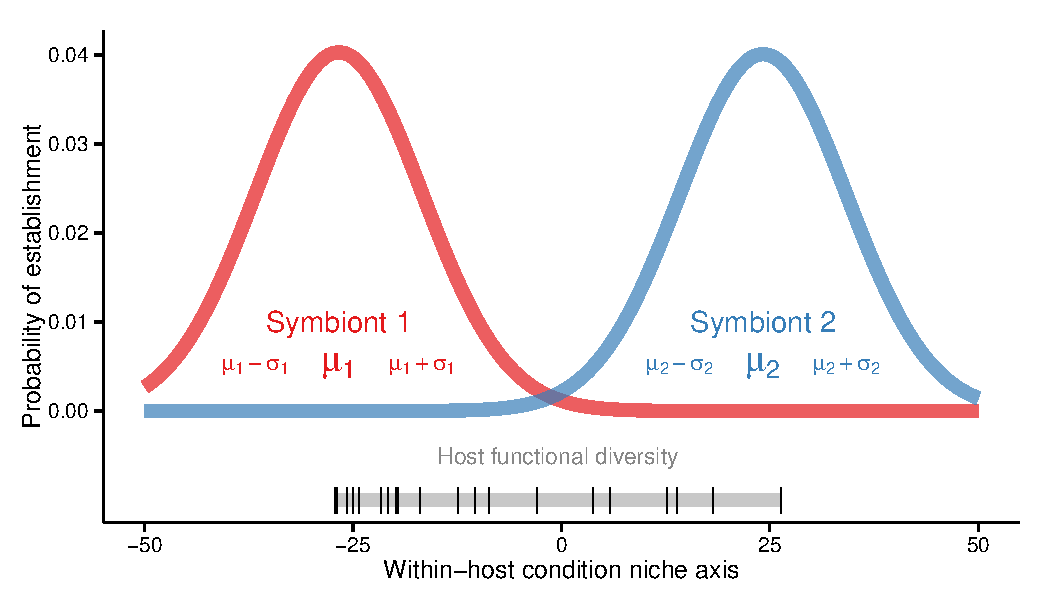
\includegraphics[width=\linewidth]{fig/niche.pdf}
\caption{Conceptual diagram illustrating the niche space of symbionts along a univariate host-condition axis (the x-axis). Each host species in a local host community is assigned one particular value, shown as vertical bars. The range of the values represents the host functional diversity represented in the local community. Here two symbiont species have equal niche breadths $\sigma$ but different optima $\mu$, which together define the Gaussian function that relates host condition to the probability of symbiont establishment, conditional on an infection attempt.}
\label{fig:niche}
\end{figure}

\newpage

\begin{figure}[ht]\centering
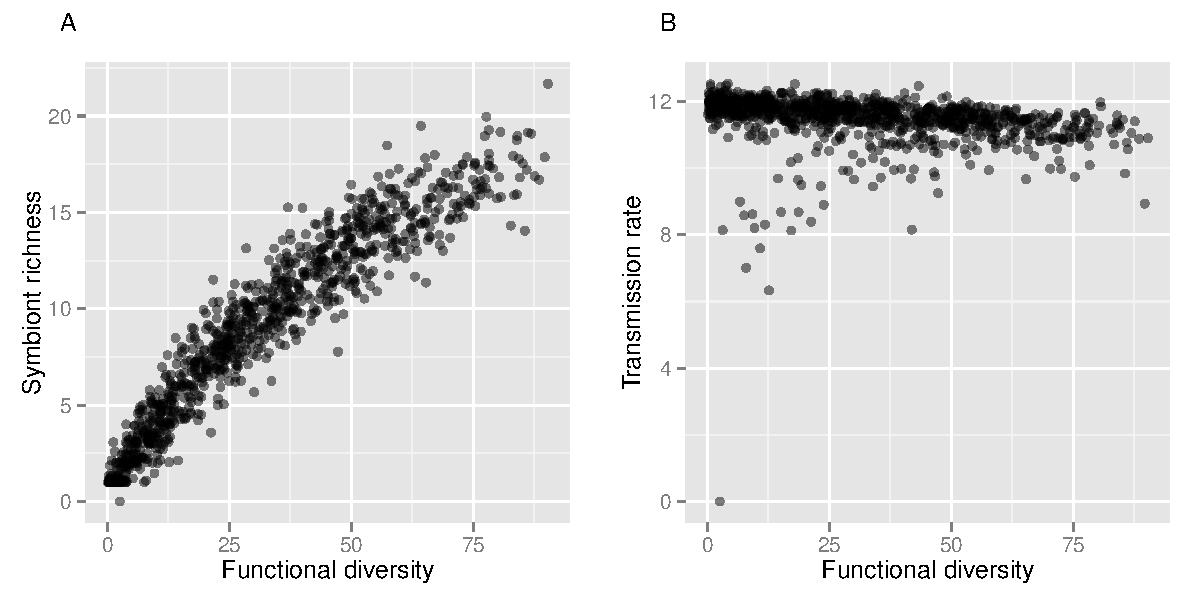
\includegraphics[width=\linewidth]{fig/fig1.pdf}
\caption{Model predictions for commensal symbionts that all have the same niche width. Panel A shows the relationship between mean host functional diversity and symbiont richness, and panel B shows the relationship between host functional diversity and symbiont transmission rate. Here, $C=500$, $H=50$, $S=50$, $\sigma = 1$, $c=0.0001$, $r=0.1$, $d=0.08$, $r_s=1$, and $\phi = 10$.}
\label{f2}
\end{figure}

\newpage

\begin{figure}[ht]\centering
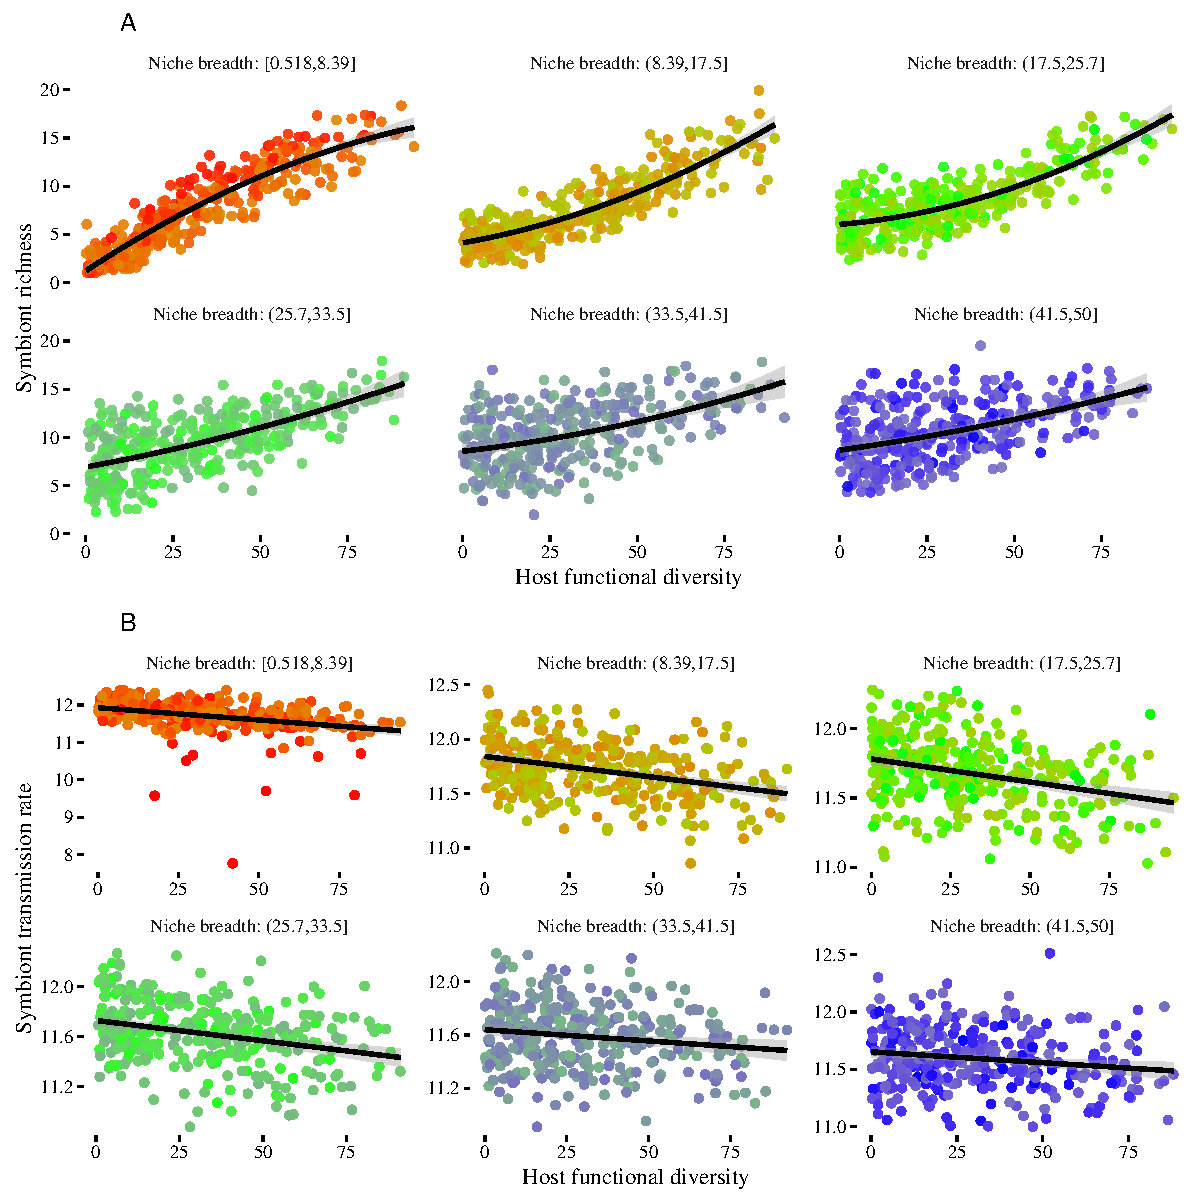
\includegraphics[width=\linewidth]{fig/fig2.pdf}
\caption{Model predictions with varying symbiont niche widths among time series (though constant within). Symbiont niche widths were uniformly generated between $\sigma_{min} = 0.5$ and $\sigma_{max} = 50$, and as before $C=500$, $H=50$, $S=50$, $c=0.0001$, $r=0.1$, $d=0.08$, $r_s=1$, and $\phi = 10$. Colors represent symbiont niche width and encode the same information as the panels, but aid in comparisons between the symbiont richness plots (panel A) and the symbiont transmission plots (panel B).}
\label{f3}
\end{figure}

\newpage

\begin{figure}[ht]\centering
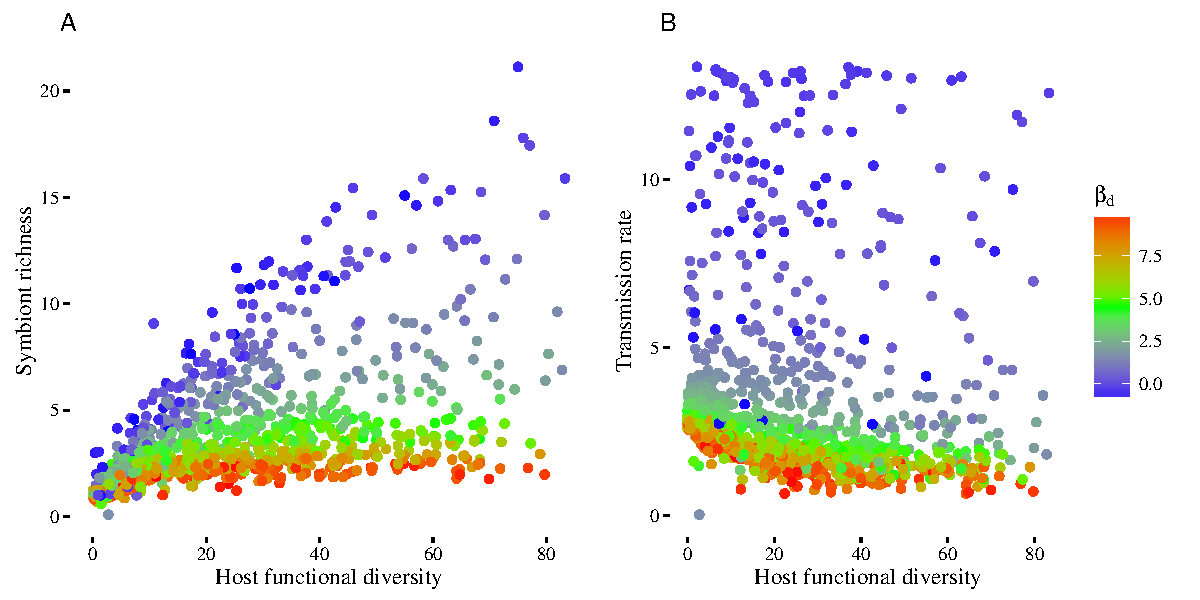
\includegraphics[width=\linewidth]{fig/fig3.pdf}
\caption{Model predictions with varying fitness consequences of infection among time series. Symbiont fitness effects $\beta_d$ were uniformly generated between $-0.99$ and $10$. Positive values of $\beta_d$ imply increased death rates with infection and more parasitic symbionts, while negative values of $\beta_d$ imply mutualistic symbionts that reduce host death rates with infection. Colors represent the particular values of $\beta_d$ selected for each simulated time series. Here, $C=500$, $H=50$, $S=50$, $\sigma = 1$, $c=0.0001$, $r=0.1$, $d=0.08$, $r_s=1$, and $\phi = 10$.}
\label{f4}
\end{figure}

\newpage

\begin{figure}
\centering
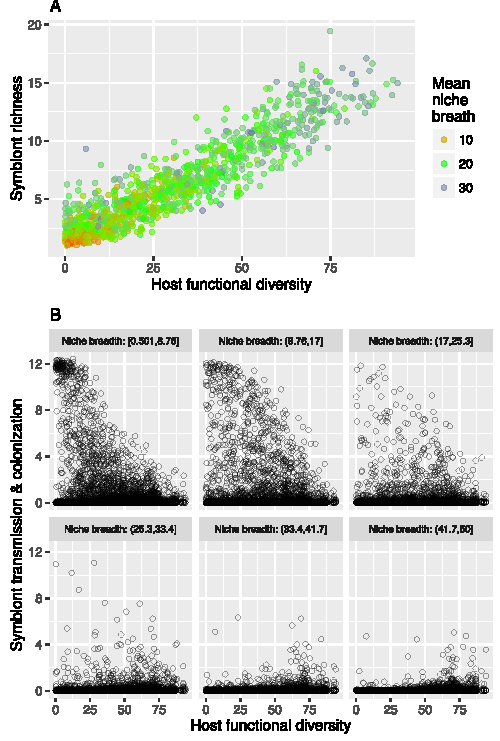
\includegraphics[width=\textwidth,height=\dimexpr\textheight-4\baselineskip-\abovecaptionskip-\belowcaptionskip\relax,
keepaspectratio]{fig/fig4.pdf}
\caption{Model predictions for mixed niche breadths within simulated time series. Here, symbiont niche breadths vary among symbiont species and are uniformly generated on the interval $(0.5, 50)$. Panel A shows the scaling of host functional diversity with symbiont richness, with the mean symbiont niche breadth in the local community shown in color. Panel B shows the transmission rates for each particular symbiont species by time series combination with panels corresponding to niche width bins. Here, $C=500$, $H=50$, $S=50$, $\sigma = 1$, $c=0.0001$, $r=0.1$, $d=0.08$, $r_s=1$, and $\phi = 10$.}
\label{f5}
\end{figure}

\newpage

\begin{figure}[ht]\centering
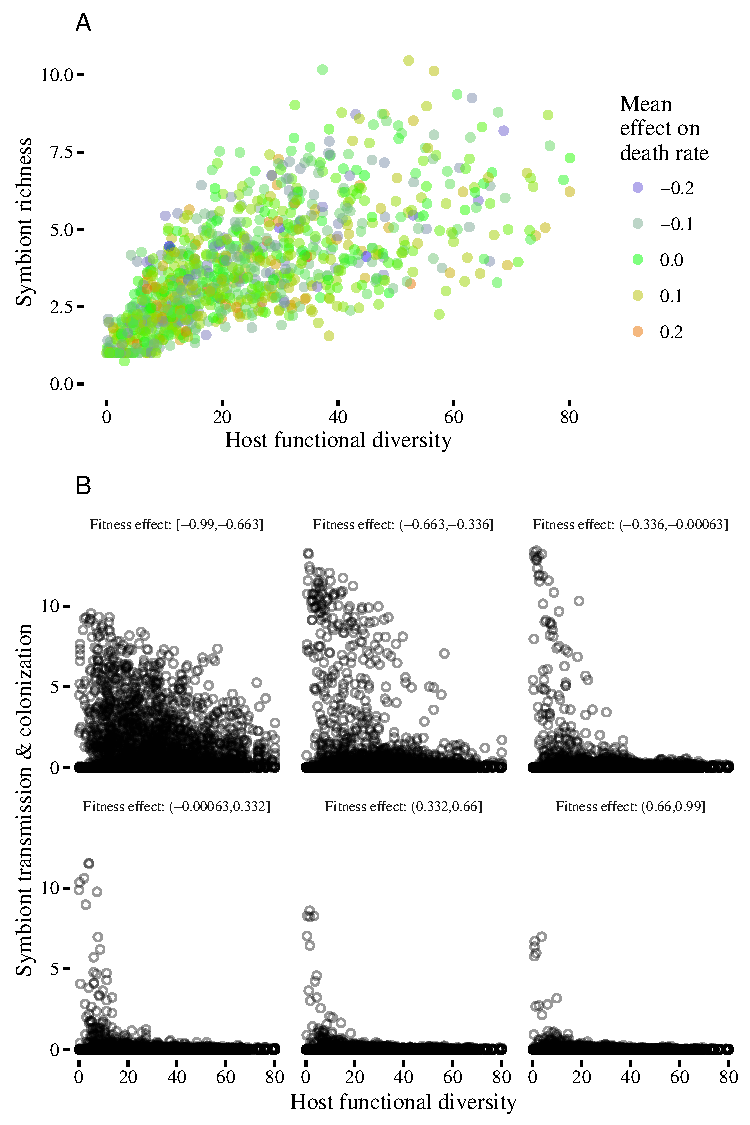
\includegraphics[width=\textwidth,height=\dimexpr\textheight-4\baselineskip-\abovecaptionskip-\belowcaptionskip\relax,
keepaspectratio]{fig/fig5.pdf}
\caption{Model predictions for mixed fitness consequences within simulated time series. Symbiont effects on the host death rate vary among symbiont species and are uniformly generated on the interval $(-0.99, 0.99)$. Panel A shows the scaling of host functional diversity with symbiont richness, and mean fitness effects are shown in color. Panel B corresponds to the transmission rates for each symbiont species in each time series with panels corresponding to death rate effect bins. If the death rate effect is negative, then infected hosts have lower death rates, surviving longer on average. If positive, hosts die faster. Here, $C=500$, $H=50$, $S=50$, $\sigma = 1$, $c=0.0001$, $r=0.1$, $d=0.08$, $r_s=1$, and $\phi = 10$.}
\label{f6}
\end{figure}

\newpage

\begin{figure}[ht]\centering
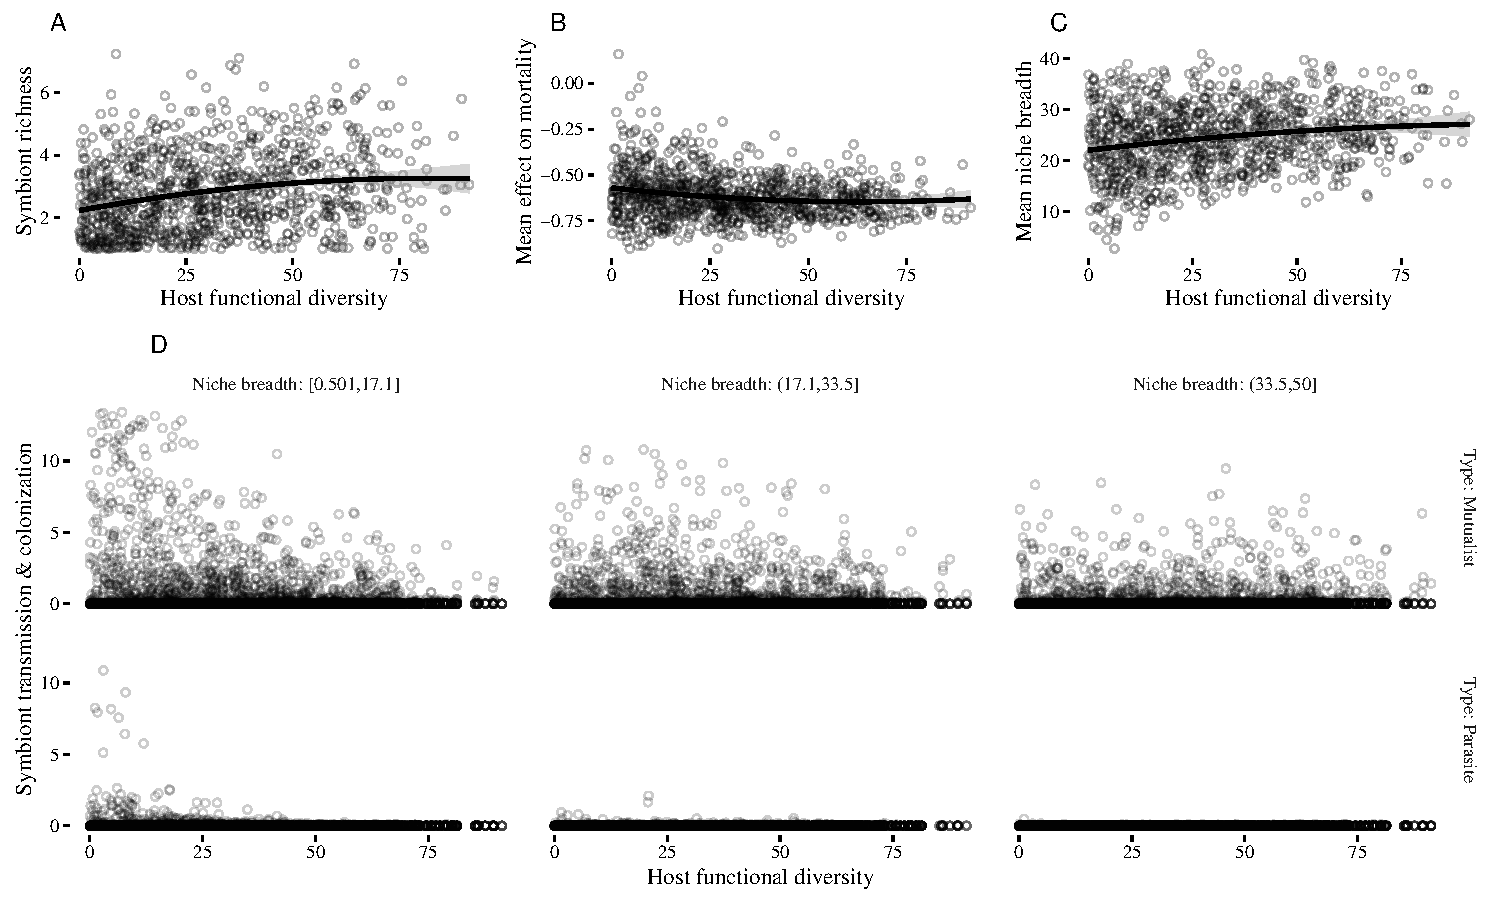
\includegraphics[width=\textwidth,height=\dimexpr\textheight-4\baselineskip-\abovecaptionskip-\belowcaptionskip\relax,
keepaspectratio]{fig/fig6.pdf}
\caption{Model predictions for mixed symbiont fitness consequences and niche breadths within simulated time series. Symbiont effects on the host death rate vary among symbiont species and are uniformly generated on the interval $(-0.99, 0.99)$, and symbiont niche breadths vary among symbiont species and are uniformly generated on the interval $(0.5, 50)$. Panel A shows the scaling of host functional diversity with symbiont richness, and mean fitness effects are shown in color. Panel B and C show the relationships between mean mortality effects and niche breadths with host functional diversity. Panel D corresponds to the transmission rates for each symbiont species in each time series with panels corresponding to death rate effect and niche breadth bins. Here, $C=500$, $H=50$, $S=50$, $\sigma = 1$, $c=0.0001$, $r=0.1$, $d=0.08$, $r_s=1$, and $\phi = 10$.}
\label{f7}
\end{figure}

\newpage

\end{document}